\begin{figure}[H]
    \centering

    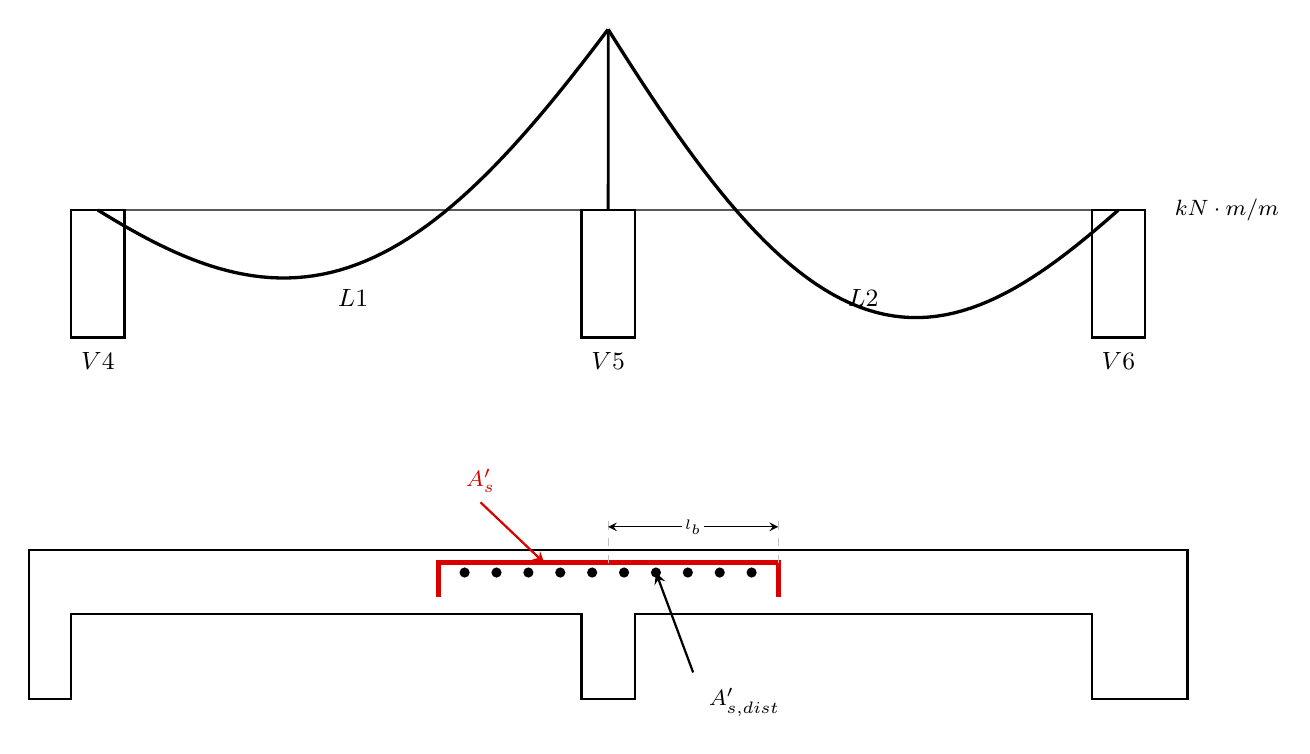
\begin{tikzpicture}[
        scale=1.35,
        pilar/.style={draw=black, thick, fill=white},
        viga/.style={line width=1pt, gray!70!black},
        linhaCompat/.style={line width=1.2pt, black},
        cota/.style={<->, >=stealth, thin, black},
        chamada/.style={gray!50, thin, dashed},
        armaduraNeg/.style={line width=1.8pt, red!85!black},
        armaduraPos/.style={line width=1.5pt, blue!80!black},
        pontoBarra/.style={circle, fill=black, inner sep=1.3pt}
    ]
    
        % --- Parâmetros de Geometria ---
        \def\L{4.8}        % Comprimento de cada vão
        \def\wP{0.5}        % Largura da viga/apoio
        \def\hP{1.2}        % Altura do apoio no diagrama superior
    
        % Coordenadas dos Apoios (V4, V5, V6)
        \coordinate (P1) at (0, 0);
        \coordinate (P2) at (\L, 0);
        \coordinate (P3) at (2*\L, 0);
    
        % ==========================================================
        % 1. DIAGRAMA DE MOMENTOS FLETORES (PARTE SUPERIOR)
        % ==========================================================
        % Eixo das Vigas
        \draw[viga] (0, 0) -- (2*\L, 0);
    
        % Apoios V4, V5, V6
        \draw[pilar] (-\wP/2, -\hP) rectangle (\wP/2, 0);
        \node[below=2pt, font=\small\bfseries] at (0, -\hP) {$V4$};
    
        \draw[pilar] (\L-\wP/2, -\hP) rectangle (\L+\wP/2, 0);
        \node[below=2pt, font=\small\bfseries] at (\L, -\hP) {$V5$};
    
        \draw[pilar] (2*\L-\wP/2, -\hP) rectangle (2*\L+\wP/2, 0);
        \node[below=2pt, font=\small\bfseries] at (2*\L, -\hP) {$V6$};
    
        % Rótulos das Lajes e Unidade
        \node[below=4pt, font=\small\bfseries, fill=white, inner sep=1.5pt] at (\L/2, -\hP/2) {$L1$};
        \node[below=4pt, font=\small\bfseries, fill=white, inner sep=1.5pt] at (1.5*\L, -\hP/2) {$L2$};
        \node[right, font=\footnotesize, fill=white, inner sep=1pt] at (2*\L + 0.5, 0) {$\text{kN}\cdot\text{m/m}$};

        % Conexão vertical do momento no apoio V5
        \coordinate (Pt2) at (\L, 1.7);
        \draw[line width=1pt, black] (\L, 0) -- (Pt2);

        % Curvas de Momento Fletor Compatibilizado
        \draw[linhaCompat] 
            plot[domain=0:\L, samples=60] (\x, {-0.95 * sin(\x * 180 / \L) + 1.7 * (\x/\L)^2});

        \draw[linhaCompat] 
            plot[domain=\L:2*\L, samples=60] (\x, {-1.35 * sin((\x-\L) * 180 / \L) + 1.7 * ((\x-\L)/\L - 1)^2});

        %\node[font=\small\bfseries, align=center] at (\L, 2.3) {Diagrama de Momentos Fletores Compatibilizados};

        % ==========================================================
        % 2. CORTE TRANSVERSAL DA LAJE E DETALHAMENTO DAS ARMADURAS
        % ==========================================================
        \def\yCorte{-3.2}     % Nível do topo da laje no corte
        \def\hLaje{0.6}      % Espessura da laje no desenho
        \def\hVigaCorte{1.4} % Altura total das vigas no corte

        %\node[font=\small\bfseries, align=center] at (\L, \yCorte + 0.95) {Corte Longitudinal da Laje — Detalhamento da Armadura Negativa};

        % Contorno de Concreto (L1 - V5 - L2)
        \draw[thick, fill=white] 
            (-\wP/2 - 0.4, \yCorte) -- (2*\L + \wP/2 + 0.4, \yCorte) --
            (2*\L + \wP/2 + 0.4, \yCorte - \hVigaCorte) -- (2*\L - \wP/2, \yCorte - \hVigaCorte) --
            (2*\L - \wP/2, \yCorte - \hLaje) -- (\L + \wP/2, \yCorte - \hLaje) --
            (\L + \wP/2, \yCorte - \hVigaCorte) -- (\L - \wP/2, \yCorte - \hVigaCorte) --
            (\L - \wP/2, \yCorte - \hLaje) -- (-\wP/2, \yCorte - \hLaje) --
            (-\wP/2, \yCorte - \hVigaCorte) -- (-\wP/2 - 0.4, \yCorte - \hVigaCorte) -- cycle;

        % Rótulos de Vigas e Lajes no Corte
        %\node[font=\small\bfseries] at (0, \yCorte - \hVigaCorte + 0.25) {V4};
        %\node[font=\small\bfseries] at (\L, \yCorte - \hVigaCorte + 0.25) {V5};
        %\node[font=\small\bfseries] at (2*\L, \yCorte - \hVigaCorte + 0.25) {V6};

        %\node[font=\small\bfseries, color=gray!50!black] at (0.35*\L, \yCorte - \hLaje/2) {Laje L1};
        %\node[font=\small\bfseries, color=gray!50!black] at (1.65*\L, \yCorte - \hLaje/2) {Laje L2};

        % --- ARMADURA NEGATIVA PRINCIPAL SOBRE V5 ---
        \def\yArmNeg{\yCorte - 0.12} % Posição superior (abaixo do cobrimento)
        \def\lAncoragem{1.6}         % Comprimento de ancoragem lb
        \def\hGancho{0.32}           % Comprimento do gancho vertical

        % Traçado da Armadura Negativa com Ganchos
        \draw[armaduraNeg] 
            (\L - \lAncoragem, \yArmNeg - \hGancho) -- 
            (\L - \lAncoragem, \yArmNeg) -- 
            (\L + \lAncoragem, \yArmNeg) -- 
            (\L + \lAncoragem, \yArmNeg - \hGancho);

        % --- ARMADURA SECUNDÁRIA (DE DISTRIBUIÇÃO - PONTOS TRANSVERSAIS) ---
        \foreach \xP in {-1.35, -1.05, -0.75, -0.45, -0.15, 0.15, 0.45, 0.75, 1.05, 1.35} {
            \node[pontoBarra] at (\L + \xP, \yArmNeg - 0.09) {};
        }

        % --- ARMADURAS POSITIVAS INFERIORES NAS LAJES L1 E L2 ---
        \def\yArmPos{\yCorte - \hLaje + 0.12}
        %\draw[armaduraPos] (0.1, \yArmPos + \hGancho) -- (0.1, \yArmPos) -- (\L - 0.1, \yArmPos) -- (\L - 0.1, \yArmPos + \hGancho);
        %\draw[armaduraPos] (\L + 0.1, \yArmPos + \hGancho) -- (\L + 0.1, \yArmPos) -- (2*\L - 0.1, \yArmPos) -- (2*\L - 0.1, \yArmPos + \hGancho);

        % --- CHAMADAS E NOTAÇÕES ---
        % 1. Armadura Negativa Principal
        \draw[<-, >=stealth, line width=0.8pt, red!85!black] 
            (\L - 0.6, \yArmNeg) -- (\L - 1.2, \yCorte + 0.45) 
            node[above, font=\footnotesize\bfseries, text=red!85!black] {$A'_s$};

        % 2. Armadura Secundária de Distribuição
        \draw[<-, >=stealth, line width=0.8pt, black] 
            (\L + 0.45, \yArmNeg - 0.09) -- (\L + 0.8, \yCorte - \hLaje - 0.55) 
            node[below right=2pt, font=\footnotesize\bfseries, text=black] {$A'_{s,dist}$};

        % 3. Gancho / Ancoragem
        %\draw[<-, >=stealth, line width=0.8pt, red!85!black] 
            %(\L + \lAncoragem, \yArmNeg - \hGancho/2) -- (\L + %\lAncoragem + 0.6, \yArmNeg + 0.35) 
            %node[above right=-2pt, font=\footnotesize\bfseries, %text=red!85!black, align=left] {Gancho / Ancoragem ($l_b$)};

        % 4. Cota do Comprimento de Ancoragem (lb)
        \draw[chamada] (\L, \yArmNeg) -- (\L, \yCorte + 0.28);
        \draw[chamada] (\L + \lAncoragem, \yArmNeg) -- (\L + \lAncoragem, \yCorte + 0.28);
        \draw[cota] (\L, \yCorte + 0.22) -- (\L + \lAncoragem, \yCorte + 0.22)
            node[midway, fill=white, inner sep=1pt, font=\tiny\bfseries] {$l_b$};

    \end{tikzpicture}
    
    %\caption{Diagrama de momentos e detalhamento da armadura negativa da laje}
    %\label{fig:detalhamento_armadura_negativa}
\end{figure}